\documentclass[portrait,a0]{sciposter}
\usepackage{ebgaramond}
\setsansfont{EB Garamond}
\usepackage{fontspec}
% Graphics stuff
\usepackage{epsfig}
\usepackage{amsmath}
\usepackage{amssymb}
\usepackage{graphicx,url}
\usepackage{tikz}
% Column stuff
\usepackage{multicol}
\setlength\columnsep{19pt}
% Unit stuff
\usepackage{siunitx}
\sisetup{
    detect-all,
    output-decimal-marker={,},
    group-minimum-digits = 3,
    group-separator={~},
    number-unit-separator={~},
    inter-unit-product={~}
}
% Tableau
\usepackage{array,multirow,makecell}
\setcellgapes{1pt}
\makegapedcells
\usepackage{booktabs}
\usepackage{blindtext}
\usepackage[inline]{enumitem}
\usepackage[english, french]{babel}
\usepackage[french=guillemets]{csquotes}
\usepackage{caption}
% Personnalisations diverses 
\addto\captionsfrench{\renewcommand{\figurename}{\textsc{Map}}}
% Force la suppression de l'espace avant ':'
 \NoAutoSpaceBeforeFDP
 
%------------------------------------------------		
% Guillemets corrects, commande G
\usepackage{xspace}
\title{\normalfont \emph{Engraved Footprints from the Past}, 29\up{th} International Cartographic Conference, Tokyo, Japan, 15–20 July 2019 - V1 (\today)}
\institute{EHESS}
%\rightlogo[1]{gfx/village.pdf}
%\leftlogo[1]{}
%\usepackage{layout}
%\usepackage{showframe}
% Réglages fins
\setlength{\parindent}{0em}
\usepackage[figureposition=top,tableposition=top]{caption}
\captionsetup{font = footnotesize, labelsep = period}
\usepackage{paracol}
%Hyper lien
\usepackage{hyperref}
%% Réglages -- Notes de BdP
%\usepackage[para]{footnotes}
\renewcommand*\footnoterule{}
\setlength{\footnotesep}{0.5cm}
\begin{document}%\layout
\makeatletter
\conference{\bf \@title}
\makeatother
\bgroup
\setlength{\parindent}{-0.1em} 
\begin{minipage}[t]{0.55\textwidth}
  \Huge
  \textsc{Engraved Footprints from the Past}\\~\\
  \Large \textsc{Retrieving Cartographic geohistorical Data from the Cassini \textit{Carte de France}, 1750 - 1789}
\end{minipage}
\begin{minipage}[t]{0.44\textwidth}
  \vspace*{-3.2cm}
  \hfill
  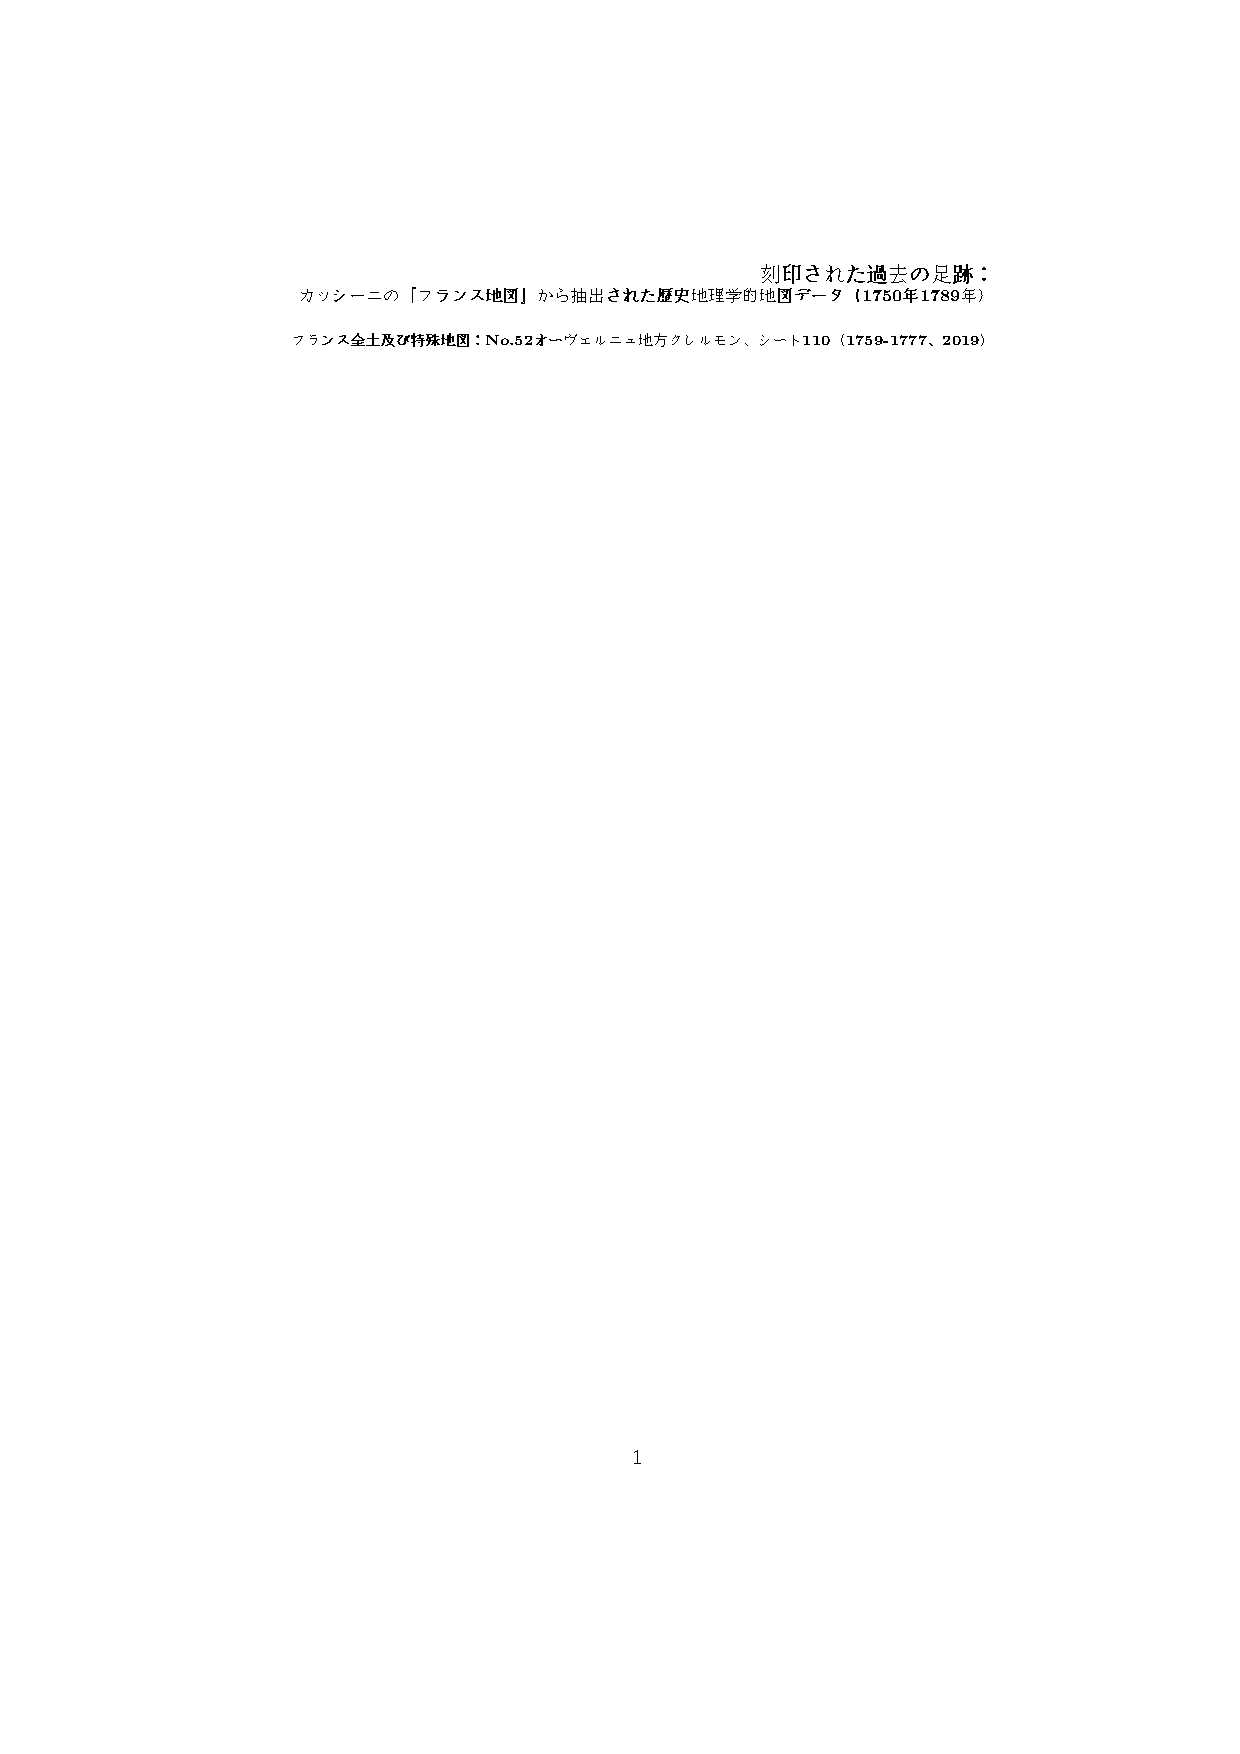
\includegraphics[width=0.95\textwidth, trim= 5cm 26cm 4cm 22cm, clip]{gfx/jap.pdf}
\end{minipage}
\egroup

\vspace{1cm}
\begin{minipage}[b]{\textwidth}
  \setlength{\parindent}{-0em}
  \begin{multicols}{3}
    \section*{\normalfont B. \textsc{Duménieu}\up{a}, J. \textsc{Chadeyron}\up{b}, P. \textsc{Cristofoli}\up{a}, J. \textsc{Perret}\up{a,c} and S. \textsc{Baciocchi}\up{a}, in collaboration with S. Gomis, M. Gribaudi, I. Langlois, C. Motte and M.-C. Vouloir
    \newline
    \noindent \tiny \up{a} EHESS, CRH, bertrand.dumenieu@ehess.fr, baciocch@ehess.fr, pascal.cristofoli@ehess.fr; \up{b} Univ. of Clermont-Ferrand (UCA), julien.chadeyron@uca.fr; \up{c} Univ. Paris-Est, LASTIG STRUDEL, IGN, ENSG, julien.perret@ign.fr
    }
    \lettrine{A}ntique maps are full of engraved geohistorical features. They provide past representations of the geographical space, favored by historians and social scientists for their uniqueness and coherence. Working on a GIS dedicated to the history of the French territory, we extracted spatial information from the Cassini \textit{Carte de France} (full name \textit{Carte générale \textsc{\textit{\&}} particulière de la France}) as vector data. Based on the first geodetic survey of France [1, 4], this well-known and monumental map has been drawn on 182 paper sheets of size 610 x 955~mm at the scale of 1:86~400 or 1 line for 100~toises (\textit{i.e.} 1 inch to 1.36 miles). It depicts the French territory with fine-grained information about populated and named places, settlements, landscape features, hydrographic, ecclesiastical and road networks [3, 5, 6, 7]. As a case study, the sheet numbered 52 provided more than \num{6800} spatial footprints that we have stored as a geographical database. Following the distinction made by Cassini himself between \og geometric \fg and \og topographic \fg entities, our geographical database is composed of two families of data, namely 1) Triangulated Geographical Entities (\og geometric \fg entities in Cassini’s own terms) whose geodetic properties are partly documented (Map. \ref{map:contours}) Relative Geographical Entities (\og topographic \fg in Cassini’s terms) which are dependent on and located relative to the former (Map. \ref{map:triangulated-relative}). Those entities are analytically distinct but come together from a same and single artifact, \emph{i.e.} the primary source they have been engraved in during the mapmaking process. Because this process of embeddedness is not fully documented, retrieving both classes of entities called for a cautious cartographic visualization with similar semiological rules and aesthetics as the original historical map. This \og Cassini map style \fg preserves the cartographic properties of the geohistorical data extracted from this primary source: generalisation, scale, spatial granularity and the overall intentions of the mapmakers [2]. Often neglected, such properties are constitutive components and dimensions of the mapping style which forms the context of and gives crucial information on the accuracy and the relationships between geohistorical data enclosed in. Our GIS-based reconstructed map (Map. \ref{GIS-based map}),  which comes with its own legend and descriptive statistics (Tab. \ref{tab:stats} and \ref{tab:symbols}), provides a renewed cartographic visualisation of the entire sheet 52. It reveals unnoticed cartographic entities that were hardly legible in the original map (Map 4a,b-e).\\
    \vfill
    \footnotesize [1] C.-F. Cassini. \textit{Description géométrique de la France}. Imp. Desaint, 1783. [2] S. Christophe, B. Duménieu, A. Masse, C. Hoarau, J. Ory, M. Brédif, F. Lecordix, N. Mellado, J. Turbet, H. Loi, T. Hurtut, D. Vanderhaeghe, R. Vergne, and J. Thollot. Expressive map design: Ogc sld/se++ extension for expressive map styles. \textit{Proceedings of the ICA}, 1:21, 2018. [3] F. de Dainville. La carte de Cassini et son intérêt géographique. \textit{Bulletin de l'Association des géographes français}, 32(251), 138-147, 1955. [4] J. V. Konvitz. Redating and rethinking the cassini geodetic surveys of france, 1730–750. \textit{Cartographica : The International Journal for Geographic Information and Geovisualization}, 19(1) :1–15, 1982. [5] C. Motte and M-C. Vouloir. Le site \href{http://cassini.ehess.fr}{Cassini.ehess.fr}: un instrument d’observation pour une analyse du peuplement. \textit{Revue du Comité Français de Cartographie}, 191, 68–84, 2007. [6] J. Perret, M. Gribaudi, M. Barthelemy, N. Abadie, S. Baciocchi, C. Bertelli, O. Bonin, P. Bordin, B. Costes, P. Cristofoli, B. Duménieu, J. Gravier, J.-P. Hubert, P.-A. Le Ny, E. Mermet, C. Motte, M. Pardoen, A.-M. Raimond, S. Robert, and M.-C. Vouloir. The 18\up{th} century Cassini roads and cities dataset, \textit{Harvard Dataverse}, 2015. [7] J. Perret, M. Gribaudi, and M. Barthelemy. Roads and cities of 18\up{th} century france. \textit{Scientific data}, 2 :150048, 2015.
    ~\\
    \begin{center}
         \captionsetup{type=figure}
      \caption{Analytical map of the geographical features surveyed for the making of the 52\up{nd} sheet of the \textit{Carte de France}, whether triangulated (316 red dots) or relative (\num{6565} grey crosses).}
      \label{map:triangulated-relative}   
      \vspace{-0.5cm}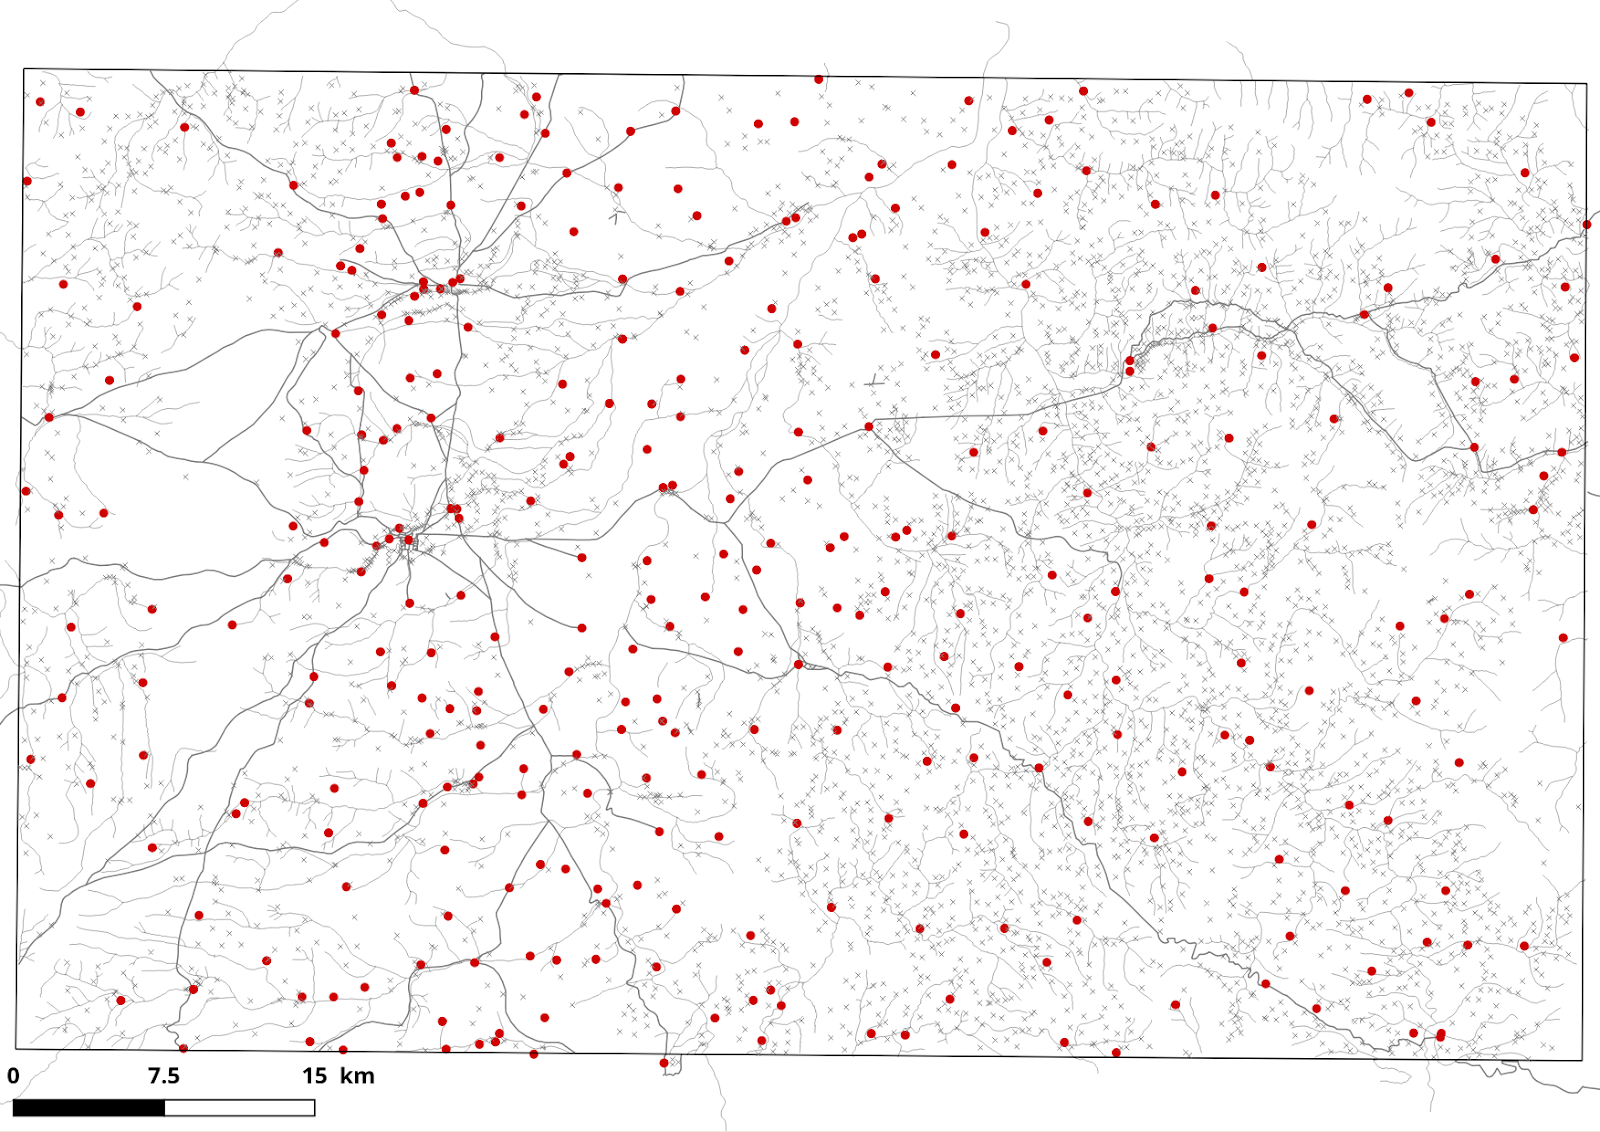
\includegraphics[width=0.9\linewidth,trim= 0cm 0cm 0cm 2cm, clip]{gfx/Triangulated.png}

    \end{center}
  \end{multicols}
\end{minipage}
%%%%

\begin{minipage}[b]{\textwidth}
  \section{\normalfont \textsc{A digital map à la Cassini: reconstruction of the \textit{Carte générale \& particulière de la France} } (2019)}
  \begin{center}
    \captionsetup{type=figure}
    \caption{Vector geographic data extracted from the georeferenced 52\up{nd} sheet of the \textit{Carte de France} rendered as a digital map mimicking the original style of the Cassini map.\protect\footnotemark}
    \label{GIS-based map}
    \vspace{-0.5cm}
    \includegraphics[width=1\textwidth,trim= 0cm 0cm 0cm 0.2cm, clip]{gfx/cassini_52_lr.png}
    \vspace{0mm}
    \footnotetext{\up{1}. The original historical map has been georeferenced, vectorised and digitally rendered at a decreased scale of 1: xx~xxx under QGIS and \LaTeX ~by the team \textsc{GeoHistoricalData} (EHESS / IGN / UCA) in 2016-2018: Nathalie \textsc{Abadie}, Stéphane \textsc{Baciocchi}, Pierre \textsc{Boivin}, Julien \textsc{Chadeyron}, Pascal \textsc{Cristofoli}, Jean-Michel \textsc{Delaveau}, Bertrand \textsc{Duménieu}, Stéphane \textsc{Gomis}, Maurizio \textsc{Gribaudi}, Isabelle \textsc{Langlois}, Claude \textsc{Motte}, Julien \textsc{Perret} \textsc{\textit{\&}} Marie-Christine \textsc{Vouloir}. Printed in Saint-Mandé, France, in January 2019 by Thierry \textsc{Chaffaud} and Régis \textsc{Fiol} at the IGN France Printed Products Manufacturing Department. With the support of the \textit{Centre de Recherches Historiques} (EHESS/CNRS), the \textit{Centre d'Histoire \og Espaces \& Cultures \fg }(UCA), the \textit{Laboratoire des Sciences et Technologies de l'Information Géographique} - LaSTIG (IGN), the \textit{Laboratoire de Démographie et d'Histoire Sociale (EHESS - Centre de Recherches Historiques)} and the SoDUCo project (ANR).}
  \end{center}
\end{minipage}
\begin{tikzpicture}[remember picture, overlay]
  \node[anchor=north west] at (0.9,6.7){%
    
\includegraphics[width=0.8\textwidth]{gfx/maplegend.png}};
\end{tikzpicture}

\vspace{-1cm}
\begin{minipage}[b]{\textwidth}
  \section{\normalfont \textsc{Retrieved geohistorical features}: descriptive statistics on the 52\up{nd} sheet of the \textit{Carte de France} (1759-1777)}
  \begin{multicols}{3}
    \setlength{\columnsep}{80pt}
    \footnotesize
    \begin{center}
      \captionsetup{type=table}
      \caption{Rectangular extent of the map in two coordinate systems: the Cassini map projection and WGS84.}
      \label{table:translation}
      \begin{tabular}{@{}lcccc@{}}
        \toprule
        & \multicolumn{2}{c}{Projected coordinates (toises)}                                                & \multicolumn{2}{c}{Geographic coordinates (degrees)}              \\
        \midrule
        & \multicolumn{1}{l}{Distance to the central meridian} & \multicolumn{1}{l}{... to its perpendicular} & \multicolumn{1}{c}{Latitude} & \multicolumn{1}{c}{Longitude} \\
        upper left corner & \num{20000}                                          & \num{162500}                                 & 45°59'9.98''N                & 2°52'23.60''E                 \\
        upper right       & \num{60000}                                          & \num{162500}                                 & 45°58'39.6''N                & 3°50'48.22''E                 \\
        bottom left      & \num{20000}                                        & \num{187500}                                & 45°32'52.36''N               & 2°50'9.38''E                  \\
        bottom right     & \num{60000}                                          & \num{187500}                                & 45°32'21.11''N               & 3°20'03.97''E                 \\
        \bottomrule
      \end{tabular}
    \end{center}
    \vfill    
    
    %\tiny{a variety of symbols mark smaller settlements: churches, wind and water mills, gallows and other works of man. Residences of nobility or gentry.
    
    %\og
    %The divided horizontal semi-circles in brass were fitted with telescopic alidades, and micrometer reading allowed angles to be observed with considerable accuracy.
    %Beacons, and sometimes lights, were used for observation marks.
    %The topographic detail was treated more summarily: though the plane table was commonly in use by the 'ingenieur géographes', the body of military surveyors, Cassini's men who carried out the minor triangulation sketched the details by estimation or by pacing, and worked this up in the office.
    %Often they were content to indicate slopes by the letters D or F ('douce' or 'forte')
    %\fg [Crone 1953:131]
    %}
    %bs%eclitartion{Triangulation \& projection}
    %\subsection{Julien}
    \footnotesize
    \begin{center}
      \captionsetup{type=table}
      \caption{Areas by land type use, lenght of hydrography and road networks }\label{tab:stats}
      \setcellgapes{2pt}
      \begin{tabular}{l|cccccccc|c|ccccc|c|c}
        & \multicolumn{8}{c|}{Landscape features}
        & Towns
        & \multicolumn{5}{c|}{Hydrography}
        & Roads
        &\\
        &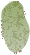
\includegraphics[height=40pt]{gfx/foret_couleur.png}
        &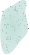
\includegraphics[height=40pt]{gfx/marais_couleur.png}
        &
\includegraphics[height=40pt]{gfx/vigne_couleur.png}
        &
\includegraphics[height=40pt]{gfx/landes_couleur.png}
        &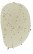
\includegraphics[height=40pt]{gfx/broussailles_couleur.png}
        & 
\includegraphics[height=30pt]{gfx/domaine_couleur.png}
        &
\includegraphics[height=35pt]{gfx/escarpement_couleur.png}
        & \rotatebox{90} {Farmland}
        &
\includegraphics[height=35pt]{gfx/ville_couleur.png}
        &
\includegraphics[height=30pt]{gfx/lac_couleur.png}          &
\includegraphics[height=25pt]{gfx/etang_couleur.png}
        &
\includegraphics[height=35pt]{gfx/riviere_large_couleur.png}
        &
\includegraphics[height=30pt]{gfx/riviere_medium_couleur.png}
        &
\includegraphics[height=30pt]{gfx/riviere_small_couleur.png}
        &
\includegraphics[height=35pt]{gfx/routes_couleur.png}
        &\textsc{Total}\\
        Features count&257&32&111&-&150&6&-&-&37&9&240&-&-&-&-&-\\
        Area sum (km\up{2})&\num{279}&\num{75}&\num{87}&\num{1368}&\num{142}&\num{0,6}&\num{0,8}&\num{1871}&\num{4}&\num{1,2}&\num{4}&\num{19}&-&-&-&\num{3852} km\up{2}\\
        % \makecell[r]{\textit{\% Map area}}&\textit{7}&\textit{2}&\textit{2}&\textit{36}&\textit{4}&\textit{0}&\textit{0}&\textit{49}&\textit{0}&\textit{0}&\textit{0}&\textit{0}&&&&\textit{100 \%}\\
        Network lenght (km)&-&-&-&-&-&-&-&-&-&-&-&-&\num{341}&\num{2841}&\num{624}&\num{3806} km 
      \end{tabular}
    \end{center}
    \vfill
    %\subsection{Pascal}
    
    %\subsection{Pascal}
    %\begin{center}
    \footnotesize
    \begin{center}
      \captionsetup{type=table}
      \caption{Map symbols census}\label{tab:symbols}
      \setcellgapes{1pt}
      \begin{tabular}{cccccccccccccccc}
        %  \hline
        % & & & & & & & & & & & & &//
        %\textsc{  Caractères géographiques   }&
        %\rotatebox{90} {\textsc{Total}} &
        %\rotatebox{90} {Villes} &
        %\rotatebox{90} {Bourgs} &
        %\rotatebox{90} {Clochers} &
        %\rotatebox{90} {Abbayes} &
        %\rotatebox{90} {Prieurés} &
        %\rotatebox{90} {Chapelles}&
        %\rotatebox{90} {Calvaires}&
        %\rotatebox{90} {Châteaux} &
        %\rotatebox{90} {Hameaux}  &
        %\rotatebox{90} {Gentillomières} &
        %\rotatebox{90} {Maisons} &
        %\rotatebox{90} {Moulins à eau} &
        %\rotatebox{90} {Moulins à vent} &
        %\rotatebox{90} {Justice} &
        %\rotatebox{90} {Autres lieux} \\
        &
        
\includegraphics[height=28pt]{gfx/ville_couleur.png}&
        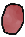
\includegraphics[height=25pt]{gfx/bourg_couleur.png}&
        
\includegraphics[height=40pt]{gfx/village.pdf}&
        
\includegraphics[height=49pt]{gfx/abbaye.pdf}&
        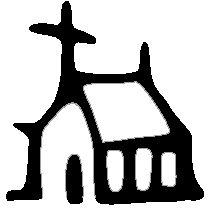
\includegraphics[height=30pt]{gfx/chapelle.pdf}&
        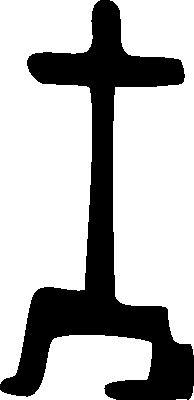
\includegraphics[height=30pt]{gfx/cross.pdf}&
        
\includegraphics[height=45pt]{gfx/chateau.pdf} &
        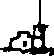
\includegraphics[height=40pt]{gfx/hameau.pdf}&
        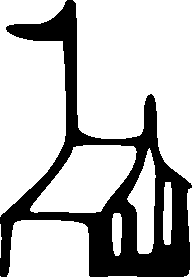
\includegraphics[height=35pt]{gfx/gentilhommiere.pdf}&
        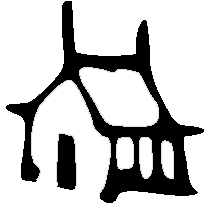
\includegraphics[height=30pt]{gfx/maison.pdf}&
        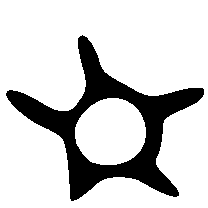
\includegraphics[height=30pt]{gfx/moulin_a_eau.pdf}&
        
\includegraphics[height=35pt]{gfx/moulin_a_vent.pdf}&
        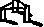
\includegraphics[height=18pt]{gfx/justice.pdf}&
        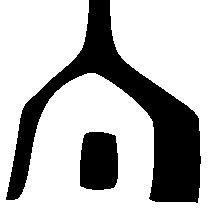
\includegraphics[height=18pt]{gfx/cabane.pdf}&
        %\textsc{Total}\\
        \textsc{Total}\\
        % \multicolumn{14}{|c|}{} \\
        % \hline
        \makecell[l]{Symbols count} & \num{15} & \num{22} & \num{234} & \num{11} & \num{93} & \num{28} & \num{196} & \num{2277} & \num{39} & \num{1135} & \num{501} & \num{1} & \num{5} & \num{6} & \num{4563}\\
        \makecell[r]{\textit{of which unnamed}} & \textit{-} & \textit{-} & \textit{1} & \textit{2} & \textit{25} & \textit{15} & \textit{46} & \textit{28} & \textit{1} & \textit{52} & \textit{427} & \textit{-} & \textit{4} & \textit{1} & \textit{\num{601}}\\
        & & & & & & & & & & & & & & & \\
        % \hline
        % \makecell[c]{\textsc{Avec toponymes}} &  &  &  &  &  &  &  &  & &  & &  &  &  & \\
        % \makecell[c]{\textsc{Sans toponyme}} &  &  &  &  &  &  &  &  &  & & &  &  &  & \\
        % \hline
        %\caption{nom du tableau}
        %\multicolumn{14}{|c|}{} \\
      \end{tabular}
    \end{center}
    \vfill
  \end{multicols}
\end{minipage}

\begin{minipage}[b]{\textwidth}
  \section{\normalfont \textsc{Primary sources, original mapmaking process \textit{\&} renewed Cassini map style}}
  \begin{multicols}{3}
    \setlength{\columnsep}{80pt}
    \textsc{Toward an in-depth reverse engineering of the Cassini map}
    \vfill
    \normalsize
    \lettrine{O}riginal 610 x 955~mm colour map (\og grand aigle \fg format) on a scale of 1: 86~400 or 1 line for 100 toises. Drawn up from 1759 to 1777 under the direction of César François \textsc{Cassini de Thury}, Charles Étienne Louis \textsc{Camus} (then Rodolphe \textsc{Perronet}) and Étienne \textsc{Mignot de Montigny}. \textbf{Triangulated from 1759 to 1775} by P.~de~\textsc{La~Court} (\textsc{ne} partial, 1759), François \textsc{Pasumot}, Claude \textsc{Pezet}, \textsc{Dallier} and \textsc{Dailley} (\textsc{no-so}, c. 1764-1766), Louis \textsc{Le~Bel} (\textsc{se}, 1766-1768; \textsc{ne} and \textsc{so}, 1769), \textsc{Dubois} \textit{\&} Louis \textsc{Cabay} (\textsc{no-ne}, 1772-1773), Q\textsc{uerry} \textit{\&} François \textsc{La~Ruelle} (\textsc{ne}, 1774-1775). \textbf{Field checked, 1767-1774} by P. \textsc{Renault} (\textsc{se}, 1767-1768), Q\textsc{uerry} \textit{\&} F.~\textsc{La~Ruelle} (\textsc{no-ne-so}, 1774). \textbf{Map engraved in Paris in 1774-1777} by Louis \textsc{Capitaine} son (for the plan, 1774-1776) and Nicolas \textsc{Bourgoin} (for the letter, 1775-1777). Printed intaglio on the press of Paris Observatory in 1777 on behalf of the \textit{Compagnie associée pour la Carte générale de la France}. Presented to the King and the Royal Court, Versailles, April 16, 1777 (\og silk printing \fg).\\
    \vfill
    \scriptsize Main primary sources: \textsc{BnF} (Paris, France) - Map division, GE C-22286 (Rés), \textit{Nouvelle carte qui comprend les principaux triangles qui servent de fondement à la description géométrique de la France, levée par ordre du Roy, par mess. Maraldi et Cassini de Thury, 1744} ; IGN France map library (Saint-Mandé, France) - Drafts of the Cassini map (sheet 52) ; Registre < A > \textit{Registre des Ingénieurs et Vérificateurs, paraphé par nous, Directeurs de la carte de France}, le 15 juillet 1778, de Montigny, f.~94, 96 et 126 ; Registre  < E > -\textit{Copie du Journal de la Carte Générale de la France tenu par M\up{r}. [Jean-Charles] de Borda [, trésorier de la Société], commencé le 26 juin 1756 et fini le 1\up{er} juillet 1784.}
    \begin{center}
      \captionsetup{type=figure}
      \caption{\scriptsize{Successive drafts of field surveys, map corrections and reviews (1759-1775)}}
      \label{map:contours}
      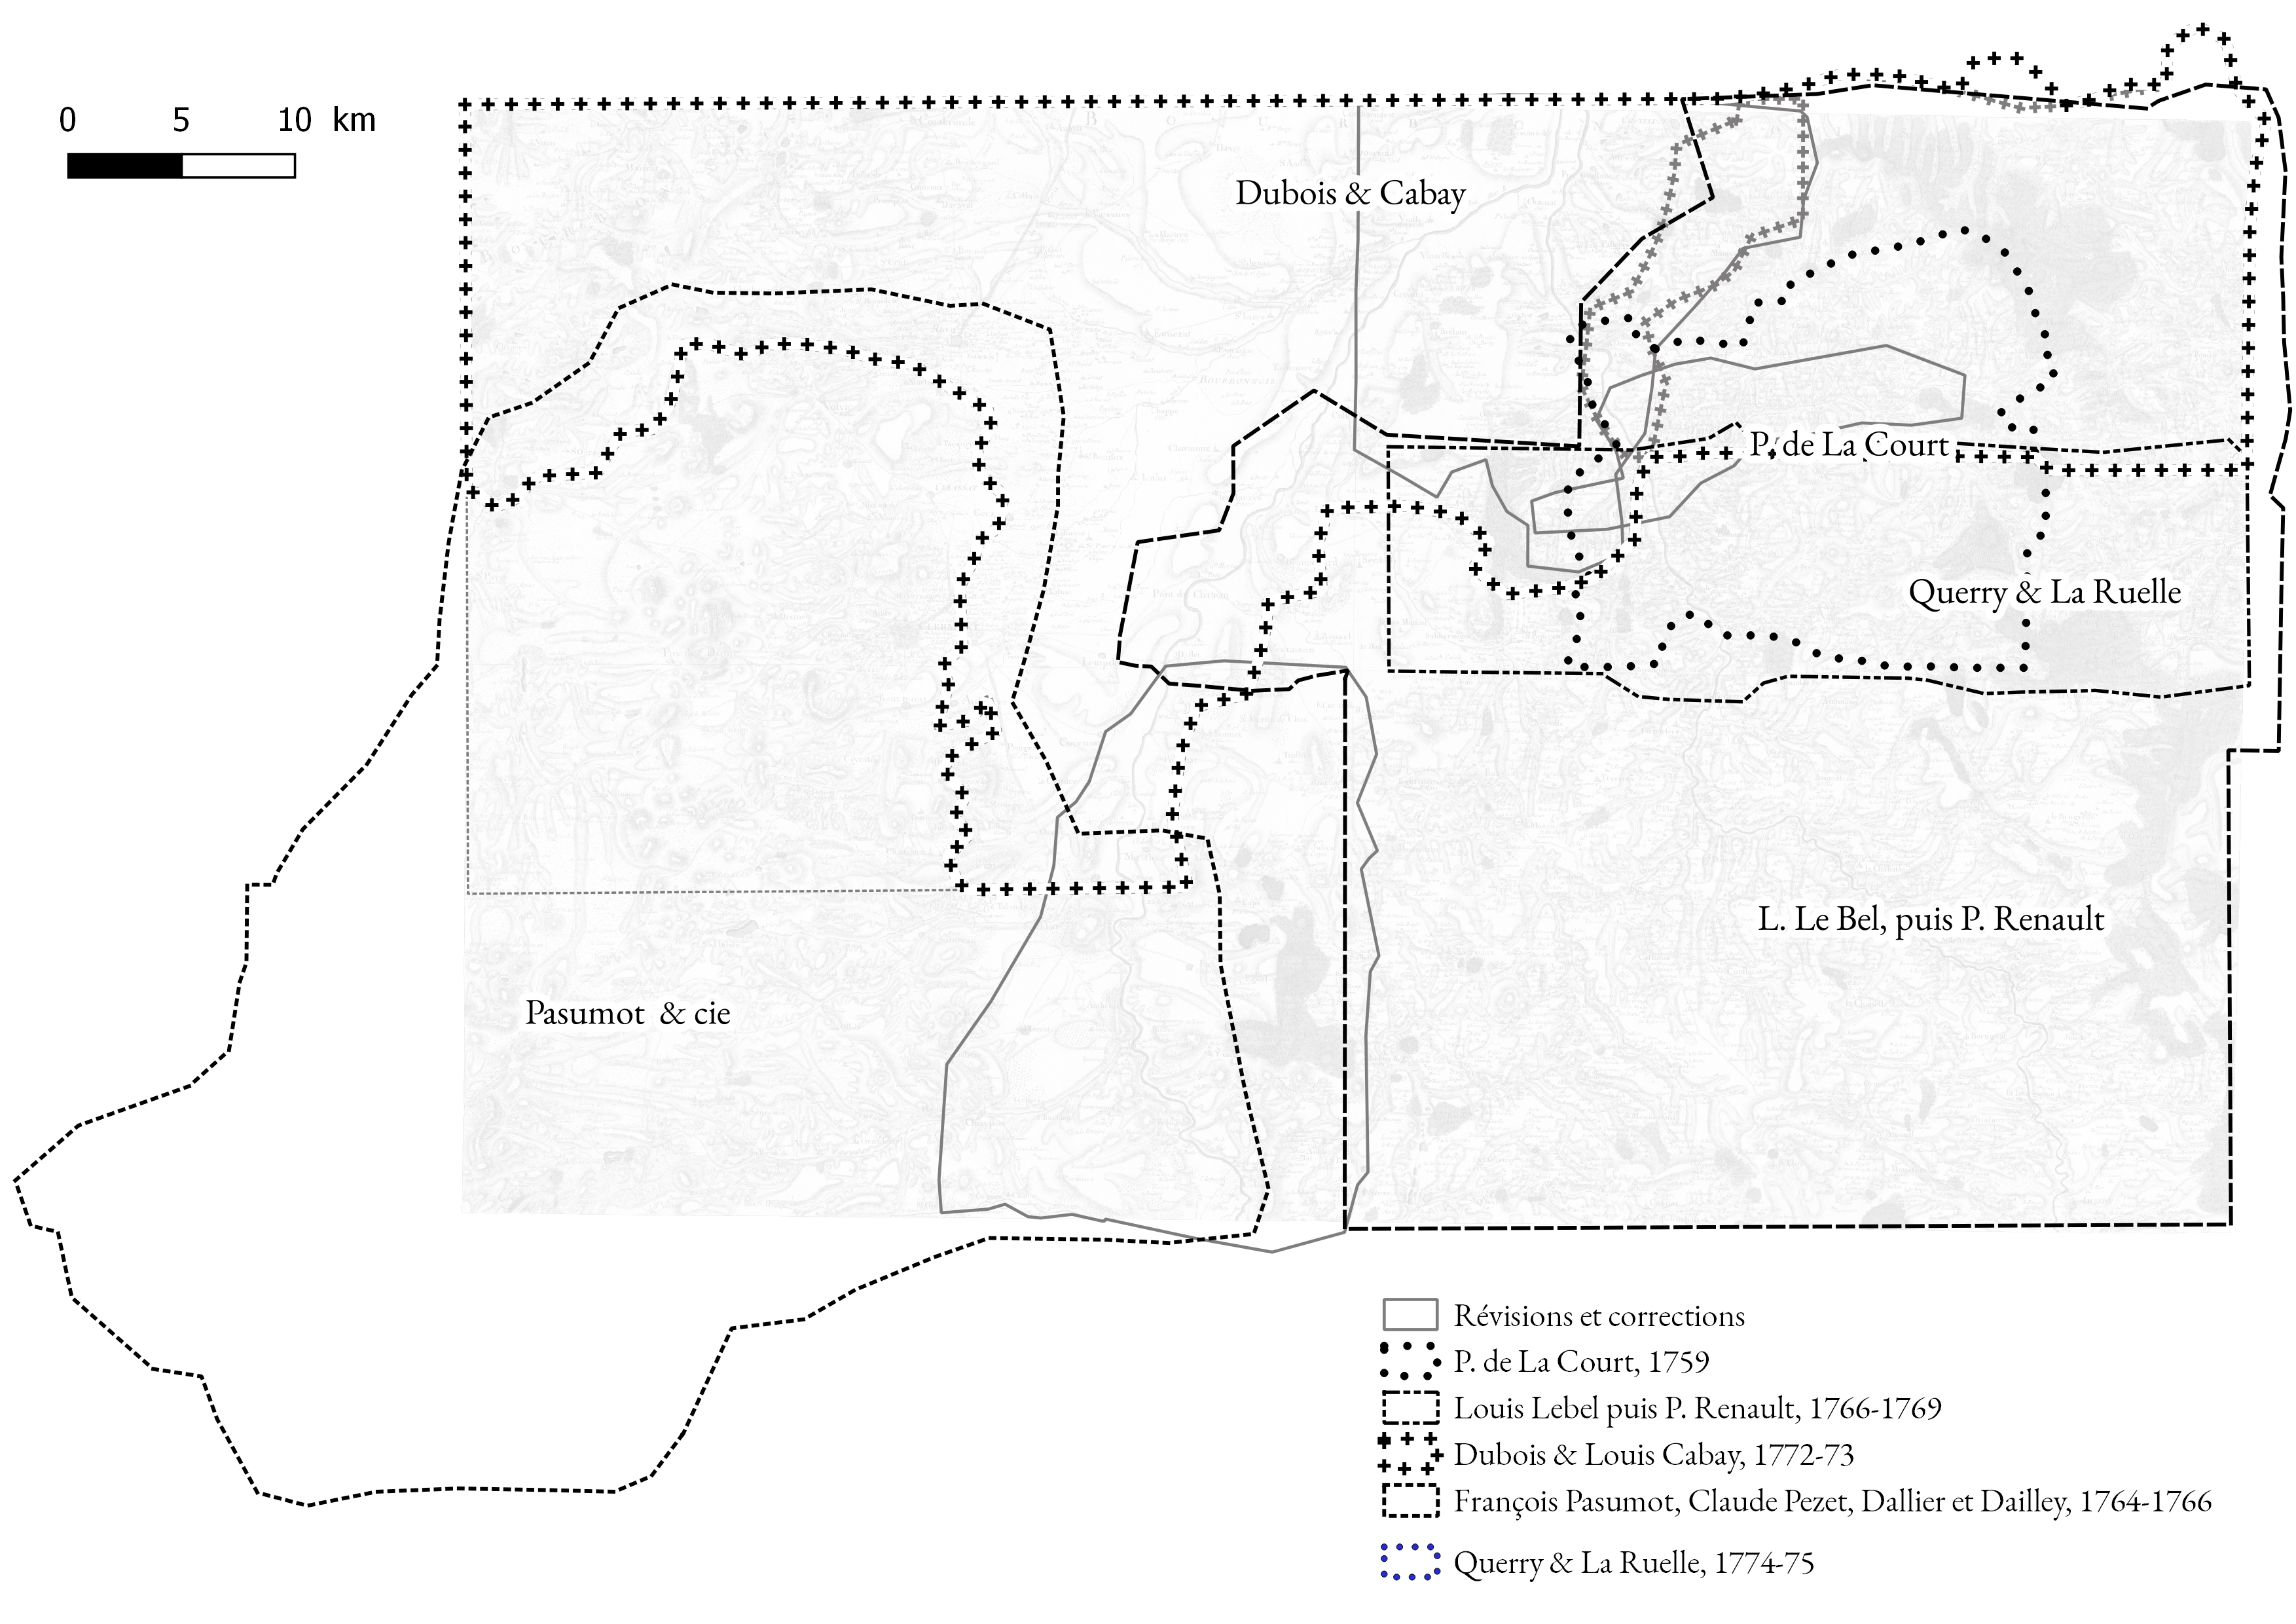
\includegraphics[width=0.28\textwidth]{gfx/Contours}
    \end{center}
~\\
    \normalsize
    \textsc{From antique to renewed GIS-based historical map}
    \vfill
    \small \lettrine{H}istoriography of cartography has long been based on critical edition of old maps published as non-georeferenced \textit{facsimile}. We propose to renew this approach by producing digital maps from vector geographic databases that combine the aesthetics and semiology of old mapping styles with the modelling capabilities of modern GIS.
    \begin{center}
     
      \includegraphics[width=0.28\textwidth]{gfx/mapmaking}
       \captionsetup{type=figure}
      \caption{\scriptsize{Vector geographic data extracted from the digitized and georeferenced original map (a) is arranged into GIS layers and composed to build the renewed version of the Cassini's Carte de France. Subfigures (b), (c) and (d) show an overview of the the 15-layers composition that results in the final rendering à la Cassini (e).}}
    \end{center}    
    
    %\scriptsize Proposition Pascal : établir la liste des couches QGis nécessaires à la construction de l'image issue de la base de donnée et les principaux problèmes liés à la conception (gérer les superpositions, la place des toponymes, le choix des couleurs, la généralisation de certains thèmes, etc...
  \end{multicols}
\end{minipage}
\end{document}
